

\chapter[A \Protege Plug-In for Editing  \FLSYSTEM Knowledge Bases]{A \Protege Plug-In for Editing  \FLSYSTEM Knowledge Bases\\
      {\Large by Aditi Pandit}}

    This chapter documents the \Protege plug-in that enables visual editing of
    \FLSYSTEM classes and instances. The plug-in appears as a tab in the \Protege
    application. Users can load \FLSYSTEM classes and
    instances into the \Protege knowledge base and then browse and edit them.
    The \Protege knowledge base can also be exported as a set of
    \fl classes and instances.

\section{Description}

The \Protege plug-in for \FLSYSTEM supports loading a \FLSYSTEM file in
the \Protege knowledge base, editing information using the \Protege
widgets, and exporting of the \Protege knowledge base as a \FLSYSTEM
file. Querying from the \Protege system and adding rules to the
\FLSYSTEM system is also supported.

For example, suppose that the following \FLSYSTEM class and instances
are loaded in module {\tt foo\_mod}:

\begin{verbatim}
foo[|
    ancestors=>person,
    age(year)=>number,
    salary(year,month)=>number
|].

john:foo.
john[age(1995)->29].
\end{verbatim}

The above \FLSYSTEM class and instance will be converted into the
\Protege classes and instances as explained in the following
paragraphs.

\underline{{\bf Representation of the class {\tt foo}}}

 The \fl class {\tt foo} is represented by \Protege class {\tt
foo@foo\_mod}, which is a subclass of {\tt :FLORACLASS}.

The \Protege class {\tt foo@foo\_mod} has slots {\tt age}, {\tt
  ancestors} and {\tt salary}, which represent the corresponding \fl
methods. It also has a slot called {\tt floraOID}. This slot is
needed to remember the OID of the corresponding \FLSYSTEM object, since
\Protege generates its own OIDs, which are different from \FLSYSTEM's.
For instance, if {\tt john:foo} is in \FLSYSTEM, then \Protege instance
of the \Protege class {\tt foo@foo\_mod} that corresponds to
(\FLSYSTEM's) {\tt john} will have \Protege OID that looks like
\emph{Kb\_0064}, but the slot {\tt
  floraOID} will have the value {\tt john}. In this way, it is possible
to associate the \Protege object \emph{Kb\_0064} with the \FLSYSTEM object
{\tt john}.

\underline{{\bf Representation of the method {\tt age}  of {\tt foo}}}

The \Protege class {\tt foo@foo\_mod} has a slot {\tt age} to represent
the \fl method {\tt age} of class {\tt foo}.  The slot {\tt age} has type
{\tt foo\_age@foo\_mod} (which is a subclass of {\tt :FLORAMETHOD}). It
has the following slots:
\begin{itemize}
\item {\tt Parameter\_year} representing the year parameter passed
to the corresponding \fl method.
\item {\tt Value\_integer}
representing the returned value of age.
\item {\tt single} representing that the \fl method returns a single value.
\item {\tt inheritable} representing the fact that the
\fl method is inheritable.
\end{itemize}


\underline{{\bf Representation of the method {\tt ancestors}  of class {\tt
      foo}}}


The \Protege class {\tt foo@foo\_mod} has a slot {\tt ancestors} to
represent the \fl method {\tt ancestors} of class {\tt foo}. The slot {\tt
  ancestors} of class {\tt foo@foo\_mod} has type {\tt
  foo\_ancestors@foo\_mod} (which is a subclass of {\tt :FLORAMETHOD}). It has the
following slots :
\begin{itemize}
\item {\tt Value\_person}
representing the returned person types.
\end{itemize}

\underline{{\bf Representation of the method {\tt salary}  of class {\tt
      foo}}}

 The \Protege class {\tt foo@foo\_mod} has a slot {\tt salary} to represent
the \fl method {\tt salary} of class {\tt foo}. The slot {\tt salary}  is
represented by an object of type
{\tt foo\_salary@foo\_mod}, which is a subclass of {\tt :FLORAMETHOD}. It
has the following slots :
\begin{itemize}
\item {\tt Parameter\_year} representing the year parameter passed
to the corresponding \fl method.
\item {\tt Parameter\_month} representing the month parameter passed
to the corresponding \fl method.
\item {\tt Value\_number}
representing the returned value of salary.
\item {\tt single} representing that the \fl method returns a single value.
\end{itemize}

\underline{{\bf Representation of the instance information}}

 Any instance of the \FLSYSTEM class {\tt foo} that is loaded into module
{\tt foo\_mod} will be represented in \Protege as an instance of
the class {\tt foo@foo\_mod}. Any method that is
declared for class {\tt foo}  will be
available as a slot of that instance. The method
will be represented in the \Protege knowledge base as an object that is
an instance of a subclass of
the special metaclass {\tt :FLORAMETHOD} as explained below.

For example, the information about the instances
\begin{verbatim}
john:foo.
john[age(1995)->29].
\end{verbatim}

will be represented using the following instances in \Protege:

\begin{itemize}
\item The \Protege class {\tt foo@foo\_mod} will have an instance with
{\tt floraOID}  having the value {\tt john}.
\item That instance
  will have a slot {\tt age}  of type {\tt foo\_age@foo\_mod}.
  This slot represents the \FLSYSTEM method {\tt age} with one argument.
  The value of this slot is an object of
  class {\tt foo\_age@foo\_mod}. This object will have an attribute
  {\tt MethodName} whose value will be {\tt john\_age\_0}.
  Numeric suffixes, such as \_0, are added to each object that represents
  a method in order to disambiguate the methods that have the
  same names but different numbers of parameters.
\item {\tt john\_age\_0} will have a slot {\tt Parameter\_year} whose value is a
  1995, and a slot {\tt Value\_integer} that has value 29.
\end{itemize}

\section{Conventions Used in Translation}
The examples of the previous section bear the marks of the complications
that one typically encounters in translating \FLSYSTEM
\FLSYSTEM knowledge bases to \Protege.
The reasons for these complications are explained below.

\begin{itemize}
\item \fl classes can be directly mapped to \Protege classes. However,
  \fl
methods cannot be directly mapped as slots of the
\Protege classes since \fl methods can take parameters, while \Protege's
  slots cannot.
\item \fl methods can be single or set valued which can be represented
as a facet in \NoProtege. However, we still needed to preserve the
distinction between inheritable and non-inheritable values.
\item The semantics of inheritance in \Protege is different from \fl.
\item \Protege internally generates OIDs for classes and instances
in it's knowledge base. These names cannot be modified in the GUI.
Hence, we need to maintain \fl instance OIDs separately.
\end{itemize}

Therefore, we used the following conventions in translating \fl classes and
instances into \Protege classes.

\begin{itemize}
\item Each \fl class is represented as a subclass of \Protege's
  class {\tt :FLORACLASS}. This
  subclass is named as {\tt floraClassname@floraModulename}.
\item Each \fl method is represented as a subclass of \Protege's class {\tt :FLORAMETHOD}. The
subclass is named as {\tt
floraClassname.methodname.number@floraModulename}. Numeric suffixes (e.g.
\_1,\_2,\_3) are used to disambiguate methods that have the same names but
different number of parameters (or different parameter types).
\item The subclass of \Protege {\tt :FLORACLASS} corresponding to the \fl class
has slots with the same names as its \fl method names in \FLSYSTEM.
\item Each instance of the \Protege {\tt :FLORACLASS}
have the slot {\tt InstanceName} whose value is the OID of the
corresponding \fl instance.
\item Each instance of {\tt :FLORAMETHOD} has a slot
  {\tt MethodName} whose value follows the following naming schema:
{\tt floraInstancename.floraMethodname.number}. Numeric suffixes 1,2,3,
  etc.,  are used to disambiguate methods that have identical names, but
  different numbers of arguments.
\item {\tt :FLORAMETHOD} subclasses have slots {\tt single} and {\tt
inheritable}, which indicate
whether the corresponding \fl method is
single or inheritable.
\item Inheritance is resolved at the \FLSYSTEM side. Each subclass of {\tt
    :FLORACLASS} shows all the methods available to it in the \Protege GUI.
  These methods may be it's own  or inherited.
\end{itemize}

The \Protege knowledge base can be edited by the user using the GUI.
However, it is important that. The above conventions are maintained.

\section{Using the \FLSYSTEM Tab}
The \FLSYSTEM tab in \Protege looks as in Figure
\ref{fig:flora-protege}:
\begin{figure}
\begin{center}
\includegraphics[height=5in,width=5in,angle=270]{flora_tab.eps}
\caption{The \FLSYSTEM tab in \Protege} \label{fig:flora-protege}
\end{center}
\end{figure}

\begin{itemize}
\item To import a set of \FLSYSTEM classes into the system, use the
Import Options box on the left side of the tab. Enter a
comma-separated list of the classes to be entered, the name of the
module in which they are to be loaded and the corresponding \FLSYSTEM
file. On hitting the import button the \FLSYSTEM classes should get
loaded into the \Protege knowledge base.

\item To export the \Protege knowledge base into a \FLSYSTEM file use
the Export Options box in the center of the left side tab. Enter the
name of the file into which to export the \Protege knowledge base
and hit the export button.

\item The \Protege knowledge base can be edited through a number of
widgets in the Class and Instance tabs of \NoProtege. When you make
changes to the \Protege knowledge base, it may become out-of-sync
with the underlying \FLSYSTEM knowledge base. To synchronize the \FLSYSTEM
system with the current state of the \Protege knowledge base hit the
Synchronize button at the bottom-left part of the tab.

\item To query the \FLSYSTEM system, use the middle box of the tab.
Enter the query and the variables to be bound. Hit the Query button
and the results will appear in the Query Results textbox. The
underlying \FLSYSTEM knowledge base is automatically synchronized when it is
queried through the GUI.

\item To add a rule to the \FLSYSTEM system, use the right-side box of
the tab. Enter the rule in the text-box and hit the Add Rule button.
\end{itemize}

\section{Class and Instance Browsers}

The class browser is shown in Figure \ref{fig:flora-cls_browser}.
The left hand side of the figure is a panel that shows the class
hierarchy, which includes the {\tt :FLORACLASS} and {\tt
:FLORAMETHOD} classes and their subclasses. The panel on the right
shows the details of all the slots (corresponding to the \FLSYSTEM
methods) for a particular {\tt :FLORACLASS}.
\begin{figure}
\begin{center}
\includegraphics[height=5in,width=5in,angle=270]{class_browser.eps}
\caption{Class browser} \label{fig:flora-cls_browser}
\end{center}
\end{figure}

The instance browser is shown in Figure \ref{fig:flora-inst1}. The
leftmost panel shows the class hierarchy. The middle panel indicates
the instances of the selected class. The rightmost panel indicates
the values of the slots of the selected instance.

\begin{figure}
\begin{center}
\includegraphics[height=5in,width=5in,angle=270]{inst_browser.eps}
\caption{Instance browser showing an instance of a \FLSYSTEM class}
\label{fig:flora-inst1}
\end{center}
\end{figure}

Figure \ref{fig:flora-inst2} also shows the instance browser, but
the selected instance is an object that represents a \FLSYSTEM method.
It shows the method name, the value, and the arguments, if
applicable.
\begin{figure}
\begin{center}
\includegraphics[height=5in,width=5in,angle=270]{mthd_browser.eps}
\caption{Instance browser showing an instance of a :FLORAMETHOD}
\label{fig:flora-inst2}
\end{center}
\end{figure}

\section{Building and Running the code}
\begin{itemize}
\item The \Protege plug-in uses the high-level JAVA interface for
\FLSYSTEM (distributed with the \FLSYSTEM system) internally. Ensure that
it is configured correctly, as described in the corresponding manual.
\item Install and configure the \Protege system from
  http://protege.stanford.edu/.
\item Configure the {\tt windowsVariables.bat} and {\tt unixVariables.sh}
  in the {\tt flora2/java} folder. Ensure that variable {\tt PROTEGE\_DIR}
  correctly points to the folder where \Protege is installed on your
  system. This folder must contain the following JAR files: {\tt
  protege.jar}, {\tt looks.jar}, 
  {\tt unicode\_panel.jar}  and {\tt driver.jar}  files.
\item Build the code using the {\tt build.bat} or  {\tt build.sh}  scripts in
the {\tt java/protegePlugin}
directory (use the appropriately changed directory for Windows). Run the
code using the scripts {\tt run\_protege.bat} or  {\tt run\_protege.sh}, as
appropriate for your system. 
These scripts are also in the {\tt java/protegePlugin} directory.
\item \Protege will run and ask you to open an old project or
configure a new one. Do as appropriate. Click on the Project menu in the
main menu bar. Select
Configure from the Project menu. A window indicating all
the plugins configured for your system will appear. Check the
box next to {\tt floraTab}. The {\tt floraTab}  will appear.
\end{itemize}

%%% Local Variables: 
%%% mode: latex
%%% TeX-master: "ergo-packages"
%%% End: 
